\begin{blocksection}
    \question Fill in each blank in the code example below so that its environment diagram is the following. Do not write any new colors (use only references to pre-existing list elements).
    
    \begin{multicols}{2}
    \begin{lstlisting}
    a = ["red", "red"]
    b = ["orange", "green", "indigo"]
    a[1] = ________
    c = ["yellow", "green"]
    a.append(______)
    c = ["blue", "violet"]
    a[___][___] = _________
    b.pop(____)
    b[1] = _________ + _________ + _________
    \end{lstlisting}
    
    \columnbreak
    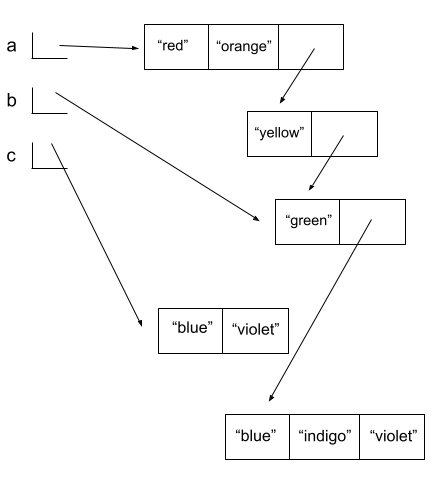
\includegraphics[width=.45\textwidth]{rainbow_connection.png}
    \end{multicols}
    
    \begin{solution}[2in]
    \begin{lstlisting}
    a = ["red", "red"]
    b = ["orange", "green", "indigo"]
    a[1] = b[0]
    c = ["yellow", "green"]
    a.append(c)
    c = ["blue", "violet"]
    a[2][1] = b
    b.pop(0)
    b[1] = [c[0]]  + [b[1]] + [c[1]]
    \end{lstlisting}
    \end{solution}
    \end{blocksection}
    
    \begin{blocksection}
    \begin{guide}
    \textbf{Teaching Tips}
    \begin{itemize}
        \item Make sure to emphasize that students cannot write new colors, i.e. they can't just say \lstinline{a[1] = "orange"}.
        \item Review with students how to use arrows in list diagrams, such as shallow and deep copies, values vs. references.
        \item The best way to approach this problem is to just go line by line.
        \item Remind your students of the order of evaluation. We can reference the old \lstinline{b[1]} to create the new \lstinline{b[1]}
    \end{itemize}
    \end{guide}
    \end{blocksection}
    